\chapter{MACHINE LEARNING-BASED RUNTIME SCHEDULER}
\label{chap:scheduler}
Rapid enhancements in computing capabilities of mobile platforms have
been driving the increased adopting and use of mobile computing
platforms by increasing numbers of users.
%
Today's mobile platforms are able to deliver capabilities that are close
to those of non-mobile platforms such as desktops or workstations.
%
For instance, a mobile phone equipped with a GPU core is able to achieve
approximately 10GFLOPS/Watt of compute-power, which is identical as a
4-core desktop with GPU~\cite{soyata}.
%
Despite of these significant advancements, mobile platforms remain
significantly limited by resources such as memory size, storage
capacity, and especially battery lifespan.
%
To alleviate the problem of the resource limitations in mobile
platforms, computation offloading techniques have been proposed as a way
to extend the capabilities of mobile platforms to more powerful
resources.
%
These may include personal computers, servers, or even public cloud
resource over the network~\cite{snarf, maui, cuckoo}.\\
%
However, the benefits from these systems can vary due to different
requirements for data transfer among various types of mobile
applications and dynamic network conditions including latency and
bandwidth.
%
As a result, offloading is not always beneficial, and poor offloading
decisions can result in the degradation of performance or energy
consumption.
%
Therefore, offloading frameworks need to consider the scheduling or
workloads onto remote or local processing resources adaptively, as a
function of network conditions and application requirements.\\
%
In this section, I address these challenges by considering machine
learning techniques for a runtime adaptive scheduler for mobile
offloading framework.
%
Machine learning technique is a branch of artificial intelligence
through which a system can learn from previous data and adapt to unseen
situations dynamically.
%
By applying machine learning techniques to the remote offloading
scheduling problem, a scheduler can be automatically trained from
previous offloading behaviors and make decisions on whether the mobile
workload should be offloaded or executed locally informed by past
behavior and current conditions.
%
There have been a number of related studies proposing adaptive
offloading mechanisms for mobile platforms.
%
To the best of our knowledge, this work is the first to systematically
study machine learning techniques for a mobile offloading scheduler.
%
To this end, I utilized the OpenCL-based offloading framework that I
explained in section~\ref{chap:offloading} and detailed measurement results
under various network conditions and mobile applications shown in
section~\ref{chap:character}.\\
%
One of the contributions described in section~\ref{chap:character} is
the combination of dynamic network conditions and application
requirements into {\it Computation to Communication ratio}, which considers
the local processing time for the workload, the amount of data transfer,
and network bandwidth.
%
The computation to communication ratio is a composite measurement which
coalesces three dynamic features into one parameter, and is used as an
attribute of the machine learning technique.
%
For the evaluation on the feasibility of applying machine learning
techniques to the adaptive scheduling problem, I utilized
{\it Weka}~\cite{weka}, a Java-based open source package.\\
%
After investigating the scheduling accuracy of several machine learning
algorithms using Weka, I choose a few machine learning algorithms which
have relatively high scheduling accuracy to implement an {\it offline}
offloading scheduler.
%
Further, by taking the complexity and scheduling performance into
account, I select Instance-Based Learning algorithm for an {\it online}
scheduler for mobile offloading framework.
%
In the evaluation, I show that although Instance-Based Learning online
offloading scheduler is fairly simple and has low overhead, it provides
performance advantages over non-adaptive schedulers for mobile
offloading system.
 
\section{Related Works}
\label{scheduler:relatedwork}
%
\subsection{Adaptive Mobile Offloading}
\label{scheduler:adaptive}
%
Many studies have considered adaptive mobile offloading
to provide performance improvements and energy savings for 
mobile platforms.
%
In~\cite{xiaohui}, the authors focus on relieving the memory limitation
of a mobile device by dynamically making the offloading decision with
Offloading Inference Engine (OLIE) which is based on the fuzzy control
model.
%
In particular, OLIE profiles the available memory size of a mobile
device and network bandwidth, and maps them into the offloading decision
specifications by the application developer, such that when the current
condition matches any specified rule, an offloading action is triggered.
%
In MAUI~\cite{maui}, the authors assume that offloading is always
preferable to local processing; however, it depends on three factors to
determine which methods should be offloaded to the remote server: the
device's energy consumption characteristics, the program characteristics,
and the network characteristics.
%
It established the relationship between CPU utilization and the energy
consumption of the mobile device and profiled the state transfer
requirement, runtime duration, and the number of CPU cycles.
%
Specifically, MAUI used the lightweight throughput measurement to profile
network condition.
%
With these information, MAUI schedules the local execution or offloading
at the beginning of the application to conserve the energy consumption
of the mobile platform.
%
In~\cite{shigeru}, a prediction model for the performance of
distributed mobile applications is evaluated through a sample image
processing application (i.e. face detection).
%
The prediction model heuristic uses linear functions to
approximate the time for local, remote execution and data transfer.
%
The server updates these functions using least-squares
method, and returns the updated heuristic linear functions to the client 
so that those updated functions are used for the performance comparison
between local processing and offloading.
%
Kovachev et al.~\cite{dejan} propose a simple cost function of
a service-based mobile cloud computing middleware for Android platforms
under three restrictions: minimized memory usage, minimized energy
usage, and minimized execution time.\\
%
Mobile "Grid" systems, where mobile devices participate as 
resource users or providers, also consider scheduling techniques to 
improve the performance of the systems while tackling the resource
constraints of mobile platforms.
%
In~\cite{waleed}, a novel energy-aware scheduling is
formulated and the level-based list scheduling heuristic is proposed for
a Mobile wireless Ad hoc NETwork (MANET).
%
The authors predefine the models for the task, the processor or the
mobile device, and the cost function, and the scheduler tries to
minimize the cost function by mapping each task to the resource through
the level-based list scheduling heuristic.\\
%
Ali et al.~\cite{hesham} present a mobile computing scheduling
mechanism based on self-ranking algorithm. 
%
Each worker node in the mobile grid system measures the connectivity and
utilization metrics and ranks itself using the ranking metric map from
the system developer.
%
Then, distributed tasks are assigned into high ranker nodes.\\
%
The distributed scheduler for the mobile grid system has
been proposed in~\cite{karin}.
%
Each mobile node self-evaluates its current and future capabilities
using static and dynamic device information such as connection quality,
remaining capacity and processor utilization, and it does matchmaking
the task requests similar to the Condor ClassAds.\\
%
Although the above-mentioned approaches take into account dynamic parameters
from the application level or the network level (i.e. CPU cycles,
network bandwidth) to predict system performance and schedule the mobile
workload execution, they still rely on predefined decision rules or cost
models, preventing the scheduler from adapting to dynamic conditions
during runtime.
%
In contrast, in this work, I consider approaches that do not rely on
any predefined specifications or prior knowledge of the mobile
application.
%
Instead, I consider machine learning techniques for adaptive runtime mobile
offloading schedulers.
%
Once trained with training data, the scheduler 
predicts the behavior of an incoming task when deciding on local or
remote execution.
%

\subsection{Machine Learning Techniques for Dynamic Scheduling Problems}
\label{scheduler:machine}
%
Machine learning techniques have been used to address dynamic scheduling
problems in various areas, such as heterogeneous computing platforms, grid
computing systems as well as in data center.
%
In~\cite{zheng}, machine learning techniques are used to provide a
compiler-based, automatic and portable predictor for multi-core
processors.
%
In order to determine the best number of threads and scheduling policy,
the authors used a feed-forward artificial neural network and a
multi-class support vector machine model, respectively.
%
Berral et al.~\cite{josep} propose an energy-aware
data center through server consolidation by turning off idle servers
with assistance from machine learning based scheduling.
%
The scheduler predicts the future performance of the jobs and power
consumption in the resulting job allocation using linear regression
algorithms.
%
The novel Adaptively Scheduled parallel R (ASpR) framework, which
transparently parallelizes scripts in the popular R language, is
presented in~\cite{jiangtian}.
%
This framework uses artificial neural networks for the performance
modeler which predicts task computation and data communication costs,
and this modeler is used by the directed acyclic graph to determine an
appropriate schedule.\\
%
In this work, I further consider the appropriateness of adopting
machine learning techniques to the scheduler of our mobile offloading
framework with respect to the complexity to construct the predictor and
ability to capture dynamic characteristics of mobile environments.
%
\section{Challenge for Adaptive Scheduling for Remote Offloading
Framework}
\label{scheduler:challenge}
In this section, I demonstrate the need for support from adaptive
runtime schedulers by conducting an experiment in which I deploy the
OpenCL-based remote offloading framework subject to various network
configurations and collect measurements to show the performance
disparity between different network configurations.\\
%
In the experiments, I utilized an Android tabletPC equipped with
1Ghz dual-core processor and 1GB RAM as a mobile client.
%
In order to observe the impact of different network
conditions on the offloading performance, I deployed a remote server
equipped with GeForce GT 640 graphics card into three different network
configurations: local area network, campus network, and Amazon EC2
instance.
%
In the local area network, I connected the mobile client and the remote
server through a wireless router supporting 802.11 b/g/n network
standard.
%
The campus network is used to represent a wide area network in which
the mobile client and the remote server are involved in different
networks: the mobile client connects to the campus wireless router and
the server connects to the laboratory internal router.
%
They communicate each other through multiple routers in the campus.
%
I used an Amazon EC2 GPU cluster as another option for the remote
server located in a wide area network, but for more restricted network
condition than the campus network.
%
Once again, Table~\ref{table:network_summary} in
section~\ref{character:setup} summarizes the average and standard deviation of latency
and bandwidth of the network configurations that I setup for the
experiments.\\
%
The benchmarks used in the experiment are sobelfilter, floating-point
matrix multiplication, Hidden Markov Model, and \textit{N}-body physics
provided by AMD APP SDK~\cite{amd} and NVIDIA~\cite{nvidia} sample code.
%
These execution kernels are used by a variety of applications in areas such as image
processing, physics simulation, and mathematical modeling.\\
%
\begin{figure}
\centering
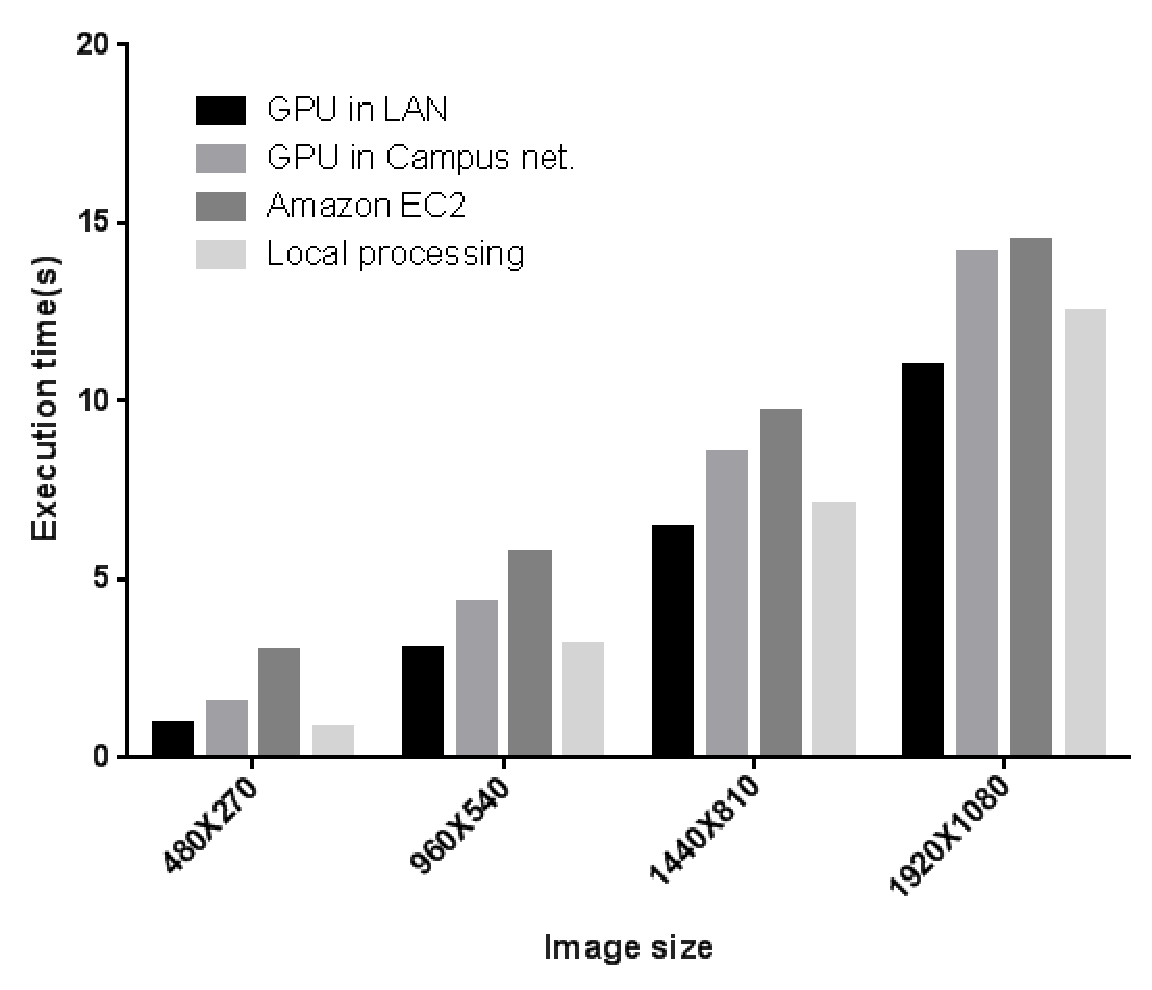
\epsfig{file=figs/challenge_network.eps, width=4.5in}
\caption{Performance for sobelfilter with various network
configurations}
\label{fig:challenge_network}
\end{figure}
%
\begin{figure}
\centering
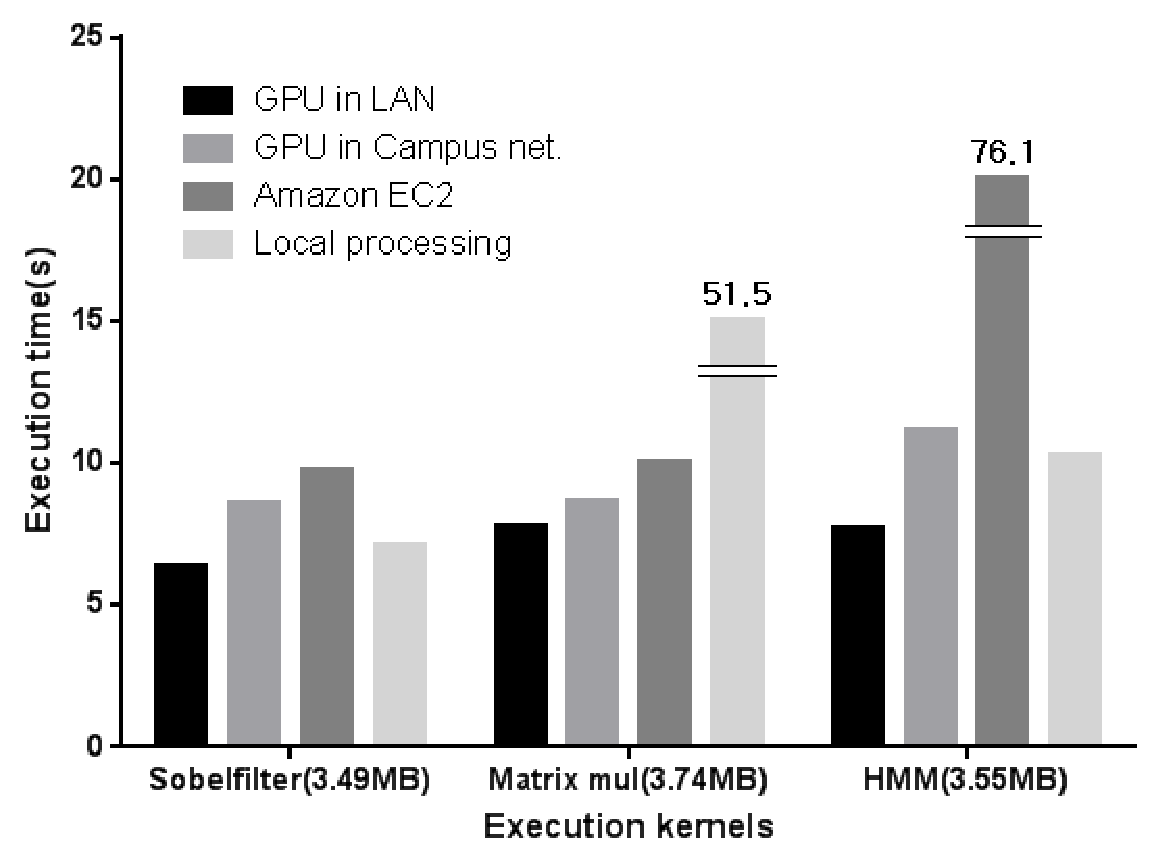
\epsfig{file=figs/challenge_workload.eps, width=4.5in}
\caption{Performance differences between various workloads}
\label{fig:challenge_workload}
\end{figure}
%
Figure~\ref{fig:challenge_network} and~\ref{fig:challenge_workload}
shows the offloading performance in terms of the
execution time compared to the case of local processing according to
the data size and network configurations for four OpenCL execution
kernels.
%
As shown in Figure~\ref{fig:challenge_network}, for sobelfilter, I observed that different
network conditions result in significantly different offloading
performance.
%
Particularly, offloading to the remote server located in a local area
network has better performance than local processing.
%
In contrast, offloading to the remote servers located in the campus network
and Amazon EC2 instance, where the offloading system has more restricted network conditions
than a local area network, takes longer time than local processing. 
%
Figure~\ref{fig:challenge_workload} shows the performance difference among various execution
workloads due to different computational requirements of workloads 
even though they process or offload the similar size of data ranging 
from 3.49MB to 3.74MB.
%
For sobelfilter, offloading to the GPU server located in LAN is only
more beneficial than local processing.
%
On the other hand, offloading floating-point matrix multiplication has
always better performance than local processing in our setup due to
heavier computational requirement of floating-point matrix
multiplication.
%
In fact, the computation complexity for floating-point matrix
multiplication is {\it O}($n^{3}$) while that for sobelfilter is
{\it O}($n^{2}$).\\
%
It is also worth noting that, for Hidden Markov Model, offloading to 
Amazon EC2 instance shows the worst performance among other cases.
%
This is because that Hidden Markov Model requires extra communications
between the mobile client and the remote server to setup additional
arguments for workload execution.
%
Packets are exchanged at higher latencies in the Amazon EC2 setup
compared with a local area network, which causes performance degradation
since our offloading framework requires that each RPC call is acknowledged 
with a response from the remote server.
%
Consequently, offloading to Amazon EC2 GPU instance, which has the
highest latency among our experimental setups, takes the longest time.
%
These results show that there is variation in offloading performance
between different network conditions and execution workloads.
%
Accordingly, proper scheduling can have a significant impact on the
offloading performance, and remote offloading framework requires the
support from the runtime scheduler.
%
\section{Machine Learning-Based Runtime Scheduler}
\label{scheduler:ml}
%
In order to apply machine learning techniques to any decision making
problems, it is first required to select a subset of relevant
attributes.
%
These need to comprehensively represent a set of problem instances in
terms of internal and external conditions which have an effect on making
a decision.
%
In this section, I describe the attributes of machine learning
techniques considered in this work, and how the proposed scheduler can
extract these attributes.
%
Then, using this subset of attributes, I investigate the scheduling
accuracy of machine learning techniques using a dataset collected from
experimental data using benchmark executions.
%
By taking the text-based dataset as an input, I can train the classifier
of various machine learning algorithms and examine the accuracy of the
trained classifiers.
%
\begin{figure}
\centering
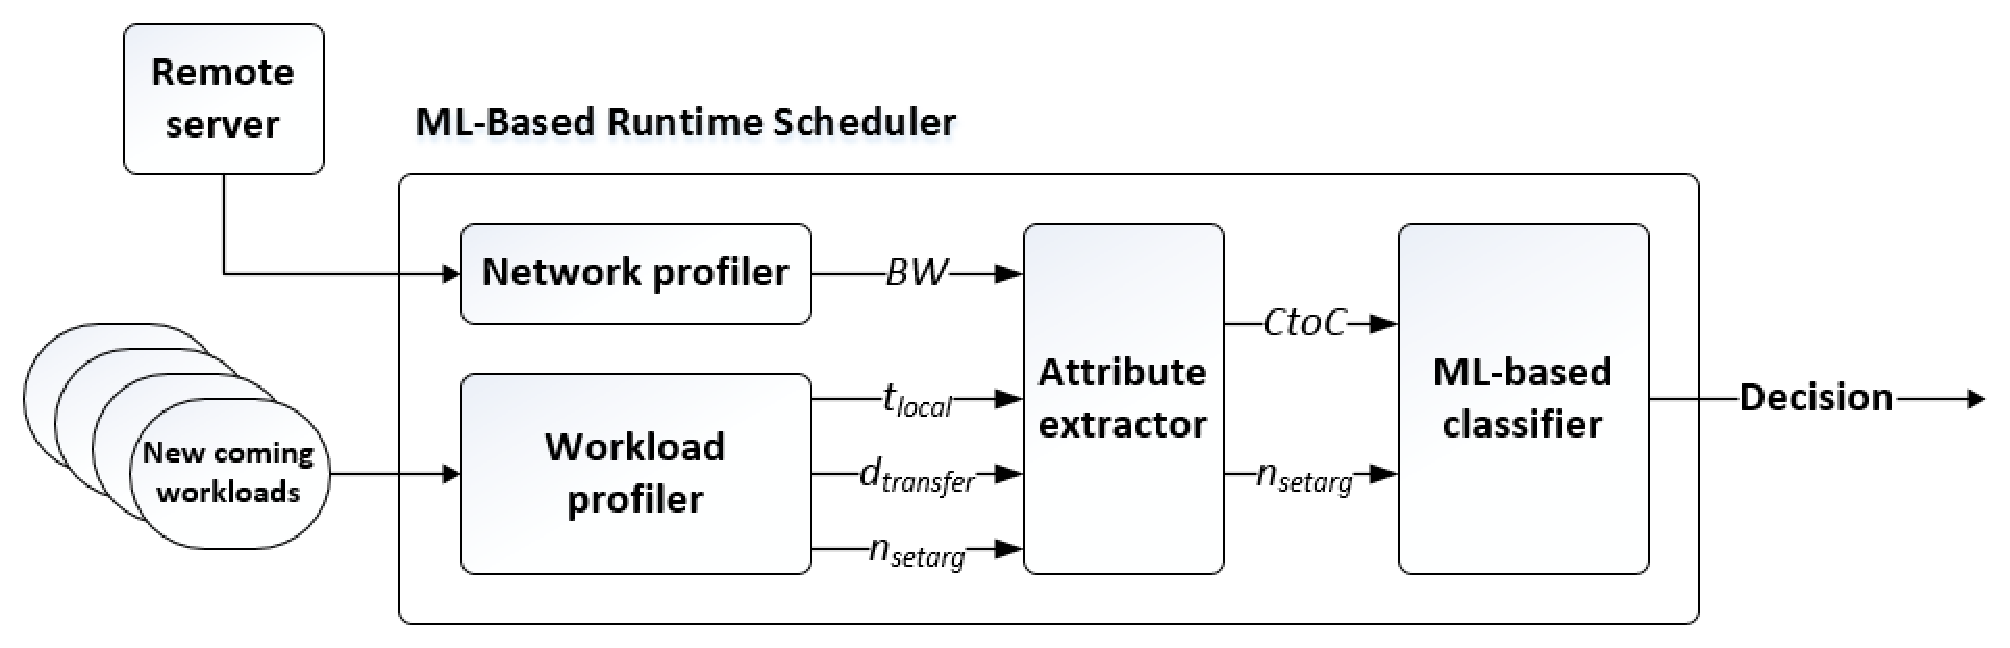
\epsfig{file=figs/scheduler.eps, width=5.5in}
\caption{Structure of machine learning-based runtime scheduler}
\label{fig:scheduler}
\end{figure}
%
Figure~\ref{fig:scheduler} illustrates the structure of the machine
learning-based runtime scheduler and how it generates and uses the
subset of attributes to make a decision for remote offloading framework.
%
\subsection{Selection of Machine Learning Attributes}
\label{scheduler:attributes}
%
Since offloading performance can vary as a function of network
conditions, the size of data to be processed, and computation
requirements, the scheduler has to take these factors into account to
make an accurate decision on offloading or local processing.
%
I focus on four features to establish the subset of attributes which is
the representation of the scheduling problem for the remote offloading
framework:1) computation amount of the workload, 2) size of data, 3)
network bandwidth, and 4) additional communication between the mobile
client and the remote resource to setup extra arguments.\\
%
{\bf Local execution time ({\it {t$_{local\_execution}$}}).} I regard the
time for a workload to be executed in the mobile client locally as the
computation amount.
%
There are a variety of methods to measure the computation amount of the
execution, such as counting the number of assembly instructions of loop
iterations, some of which require additional assistance from the
special hardware or compiler.
%
Instead, in the proposed approach, runtime measurements are taken by the
offloading framework as it executes the workload with the given data
locally, and the scheduler profiles the execution time for the
workload.\\
%
{\bf Data size to be transferred ({\it {d$_{transfer}$}}).} In addition
to the computation cost of a workload depending on the size of the data,
the data size also affects the communication cost to transfer the data
from the mobile client to the remote resource.
%
In the OpenCL-based remote offloading framework, the APIs for buffer
management such as {\it clEnqueueWriteBuffer} and {\it
clEnqueueReadBuffer} are used to profile the size of data to be
transferred.\\
%
{\bf Network bandwidth ({\it BW}).} I integrate the network bandwidth
measurement into the offloading framework so that it is able to measure
network bandwidth between the mobile client and the remote resource
during runtime.
%
In the implementation, network bandwidth is simply measured by the size
of probing packets divided by the elapsed time to send those
packets~\cite{bandwidth}.\\
%
{\bf Number of the invocations for argument setup ({\it
{n$_{arguset}$}}).} I count the number of the invocations of the specific
OpenCL API called {\it clSetKernelArgs}, which causes additional
communication overhead between the client and the remote resource to
setup the extra arguments for kernel executions in addition to the
primary data setup.
%
The reason why I distinguish communications between main data transfer
and additional arguments setup is that, though the latter incurs minor
amount of data, it can cause significant communication costs due to
protocol round-trip messages between the client and the remote
resource.\\
%
Not that, rather than considering the local execution time, the size of
data transfer, and network bandwidth as individual attributes
separately, I use {\it Computation to Communication ratio} in which
three features are merged into one attribute as Equation~\eqref{equ:ctoc}.
%
\begin{equation}
\begin{split}
	CtoC& = t_{local\_execution}\:/\: t_{data\_transfer} \\
	& = t_{local\_execution}\:/\:(d_{transfer}\:/\:BW)
\end{split}
\label{equ:ctoc}
\end{equation} 
%
where {\it t$_{data\_transfer}$} is the time for data transfer.
%
Thus, in this work, computation to communication ratio is a composite
measurement which combines three dynamic features into one parameter.
%
As a result, the proposed machine learning-based classifier accepts two
attributes: computation to communication ratio({\it CtoC}) and the
number of invocations of {\it clSetKernelArgs}({\it n$_{argset}$}) to
make a decision on scheduling a new workload(i.e. local processing or
remote offloading).
%

\subsection{Scheduling Accuracy of Machine Learning techniques}
\label{scheduler:accuracy}
%
In this subsection, I investigate the scheduling accuracy of the machine
learning-based scheduler for remote offloading framework.
%
First of all, by running the OpenCL-based offloading framework into the
experimental setup with various network configurations, execution
kernels, and data sizes as described in
section~\ref{character:methodology}, I gathered a total 640 data
instances to train and test the classifiers of various machine learning
algorithms.
%
Each data instance means one execution of the offloading framework, and
consists of \{{\it d$_{transfer}$}, {\it BW}, and {\it n$_{argset}$}\}.
%
Next, I aggregate collected data instances to create the training and
test datasets, each consisting of a 3-tuple, {{\it CtoC}, {\it
n$_{argset}$} ; {\it label}}, with two attributes explained in
section~\ref{scheduler:attributes} and the label which is a decision on
{\it offload} or {\it local}.
%
\begin{figure}
\centering
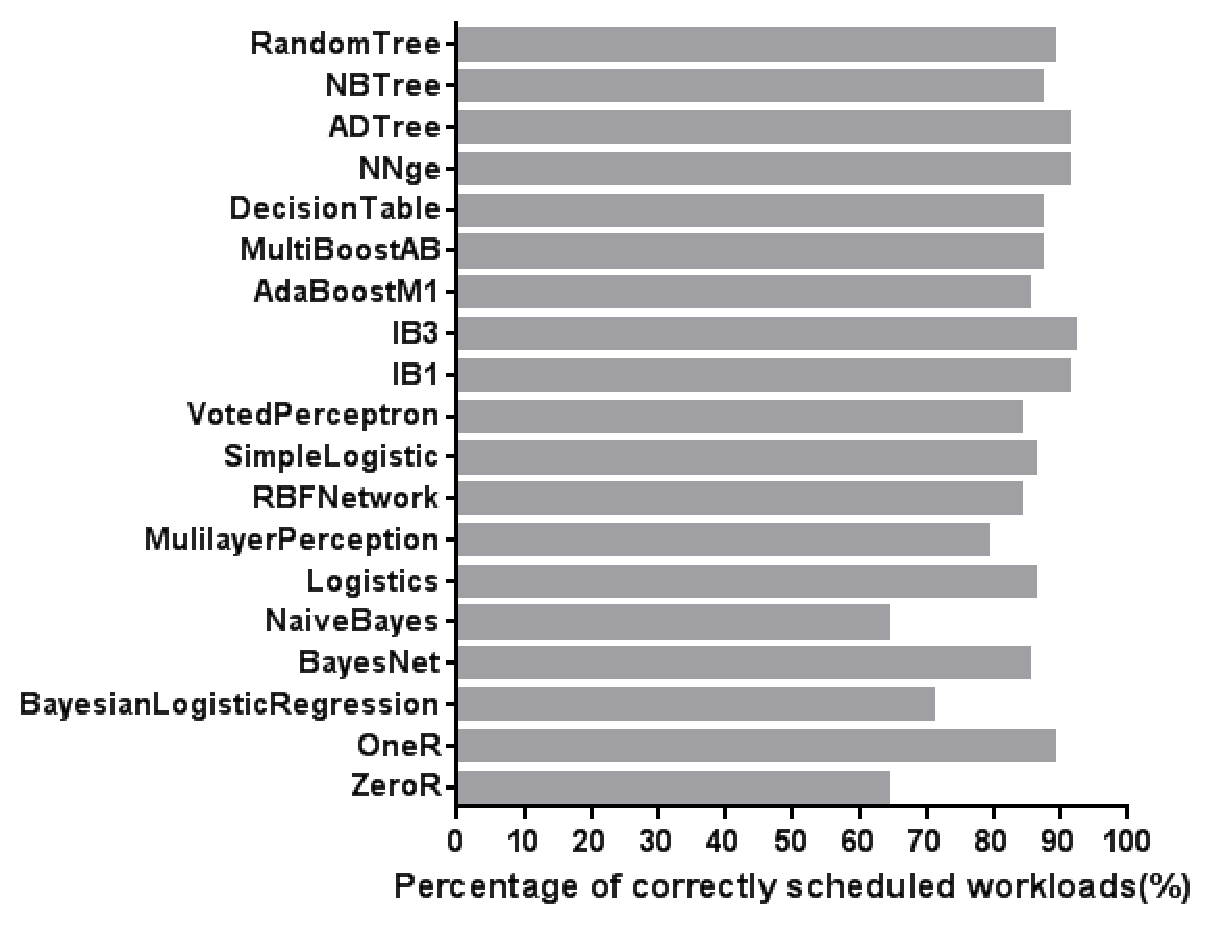
\epsfig{file=figs/scheduling_accuracy.eps, width=4.5in}
\caption{Offloading scheduling accuracy of various machine learning
algorithms}
\label{fig:scheduling_accuracy}
\end{figure}
%
Then I labeled each data instance by comparing offloading 
performance to the local execution in terms of the execution time.
%
For example, if offloading sobelfilter with a 1920$\times$1080 image
into a machine with a GPU in LAN takes a shorter time than
local processing, the instance is labeled as \textit{offload}.
%
In the collected dataset, 65\% of instances are labeled as
\textit{offload}.
%
Note that it is possible to use another performance metric: mobile
device's energy consumption, such that each instance can be labeled
based on energy consumption between remote offloading and local
processing.
%
Lastly, I separated the collected dataset with 70\% of them for
the training dataset and the rest for the test dataset, so they have
the identical distribution for instance properties.\\
%
Using the training dataset, I trained the classifiers of various
categories of machine learning algorithms such as Decision Tree,
Bayesian Networks, Instance-Based Learning, and Perceptron-Based
Learning. 
%
In the training phase, Weka takes the text-based training dataset as
the input and automatically generates the classifier associated with
each machine learning algorithm.
%
Once each classifier is trained, I tested the accuracy of the
trained classifier with the test dataset by observing whether the
trained classifier labels each instance in the test dataset correctly or
not.\\
%
Figure~\ref{fig:scheduling_accuracy} shows the scheduling accuracy of
various machine learning algorithms.
%
In this evaluation, the scheduling accuracy is calculated through the
number of the correct decisions made by the classifier out of the test
dataset.
%
I observed that two Instance-Based Learning classifiers performed 
the most accurate prediction, showing greater than 90\% of the scheduling
accuracy.
%
The basis for the classification of Instance-Based Learning is the instances 
database, where previously seen instances are stored.
%
Instead of building the explicit classifier as other machine learning
algorithms, Instance-Based Learning compares a new problem instance with the stored
instances in the database to select {\it k} most similar instances 
from the database and votes the majority of the selected instances to 
predict the label of the new problem instance.
%
{\it k} set to 1 (IB1) and 3 (IB3) as higher values showed the same
performance. 
%
The classification of probabilistic machine learning
techniques such as Bayesian Networks is based on the statistics
of attributes of the previous instances such as the mean and the
variance values.
%
Thus it is possible that probability-based machine learning
algorithms overlook the edge of previously seen instances, which causes
the performance degradation for the prediction problem. 
%
In fact, Naive Bayes has the worst performance among machine learning
algorithms used for the evaluation, showing 64.4\% scheduling
accuracy.
%

\section{Performance Evaluation for Offline Scheduler}
\label{scheduler:offline}
%
In this section, using the classifiers from various machine learning
algorithms, I implement an offline offloading scheduler and evaluate
the performance and penalty of the offline runtime schedulers.
%

\subsection{Experimental Setup}
\label{schedeulr:offline_setup}
%
Based on scheduling performance and algorithm complexity, I selected
three machine learning algorithms: RandomTree, Instance-Based Learning
and Rule-Based Learning, and built them onto our remote offloading
framework for the offline runtime scheduler.
%
For RandomTree, I used the classifier that Weka generated using the
training dataset described in section~\ref{scheduler:accuracy}.
%
Total depth of the tree is 101 and the scheduling accuracy simulated
through Weka is 89.5\%.\\
%
Though I do not need any classifier for Instance-Based Learning
algorithm, it is required to define the similarity between a new problem
instance and previously stored instances in the database.
%
To do this, I used Euclidean distance, which is common to measure the
similarity for Instance-Based Learning~\cite{instance}.
%
The closer the distance between instances is, the more similar 
they are.
%
I stored the training dataset with 448 instances to build the
database for the Instance-Based Learning algorithm.
%
For simplicity, I use {\it k=1} for Instance-Based Learning
algorithm.
%
For Rule-Based Learning, I establish a simple rule based on
computation to communication ratio threshold, in which the scheduler
decides to offload the mobile computation only if
computation to communication ratio is higher than the threshold.
%
Based on our observation, it is most likely that the benefits from
offloading are more promising when computation to communication ratio is
higher than 1.5.
%
For that reason, I setup the threshold with 1.5 and 3.\\
%
Also, I emulate various network configurations in which the
client and the server connect directly through a wireless router, but
have 9 different network bandwidths ranging from 6.5MB/s to 0.3MB/s
controlled by Traffic Control (TC)~\cite{tc}.
%
TC is a network tool which provides functionalities to control network
traffic by prioritizing network resources and using concepts of traffic
classification, queue disciplines and quality of service (QoS).
%
While setting different network bandwidths, I ran
our offloading framework with four benchmark kernels 720 times (9
network bandwidths $\times$ 4 kernels $\times$ 4 data sizes $\times$ 5
repeats for average) per each offline scheduler.
%

\subsection{Performance Comparison}
\label{scheduler:offline_perf}
%
\begin{figure}
\centering
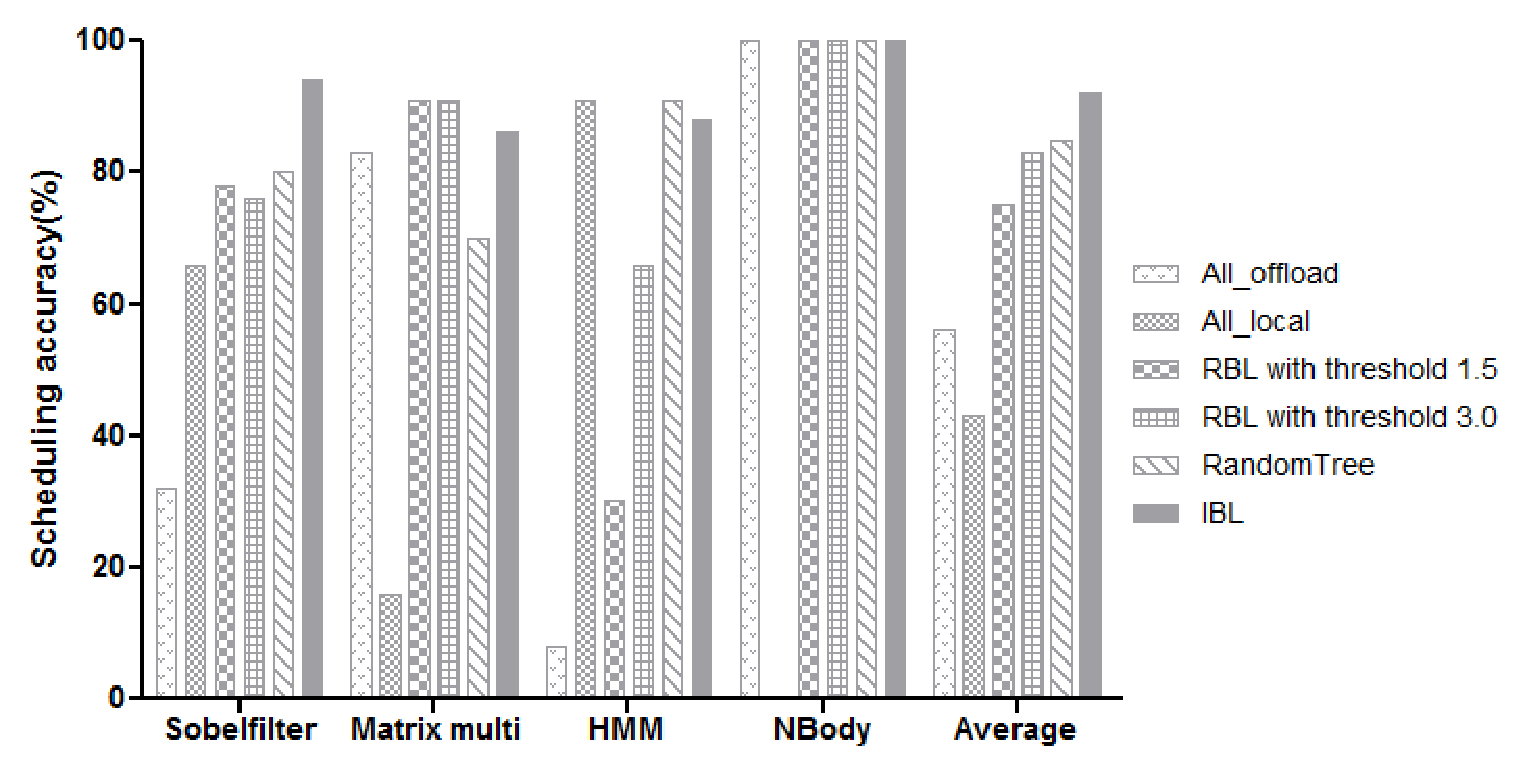
\epsfig{file=figs/offline_accuracy.eps, width=5.5in}
\caption{Scheduling accuracy of offline schedulers}
\label{fig:offline_accuracy}
\end{figure}
%
Figure~\ref{fig:offline_accuracy} shows the scheduling accuracy for various machine learning
algorithms with four benchmark kernels.
%
Similarly as the result shown in Figure~\ref{fig:scheduling_accuracy}, I observed that
Instance-Based Learning has the most accurate scheduling performance
among various schedulers showing 92\% of the scheduling accuracy.
%
Even though in matrix multiplication and Hidden Markov Model,
other machine learning algorithms have better performance than Instance-
Based Learning, Instance-Based Learning shows the best performance on average.
%
It is also observed that, even though the schedulers based on Rule-Based
Learning algorithm consider only one attribute,
computation to communication ratio, they have better performance than
RandomTree.
%
An interpretation is that the computation to communication ratio is a
more dominant attribute than the number of argument setup, {\it n$_{argset}$}.
%
Interestingly, for {\it N}-body physics, all machine learning
algorithms show the perfect scheduling accuracy.
%
It is because that computation to communication ratio for
{\it N}-body physics is extremely high in our experimental setup
so that it is easy for the scheduler to differentiate the conditions 
where offloading or the local execution for {\it N}-body physics 
is more beneficial than the other.
%
In fact, offloading {\it N}-body physics always had better
performance that the local execution in the experimental setup.\\
%
Figure~\ref{fig:penalty_time} and~\ref{fig:penalty_energy} 
present the penalty for various schedulers
normalized to the case of the oracle scheduler which always makes the
right decision to offload or run locally as Equation~\eqref{equ:penalty}.
%
\begin{figure}
\centering
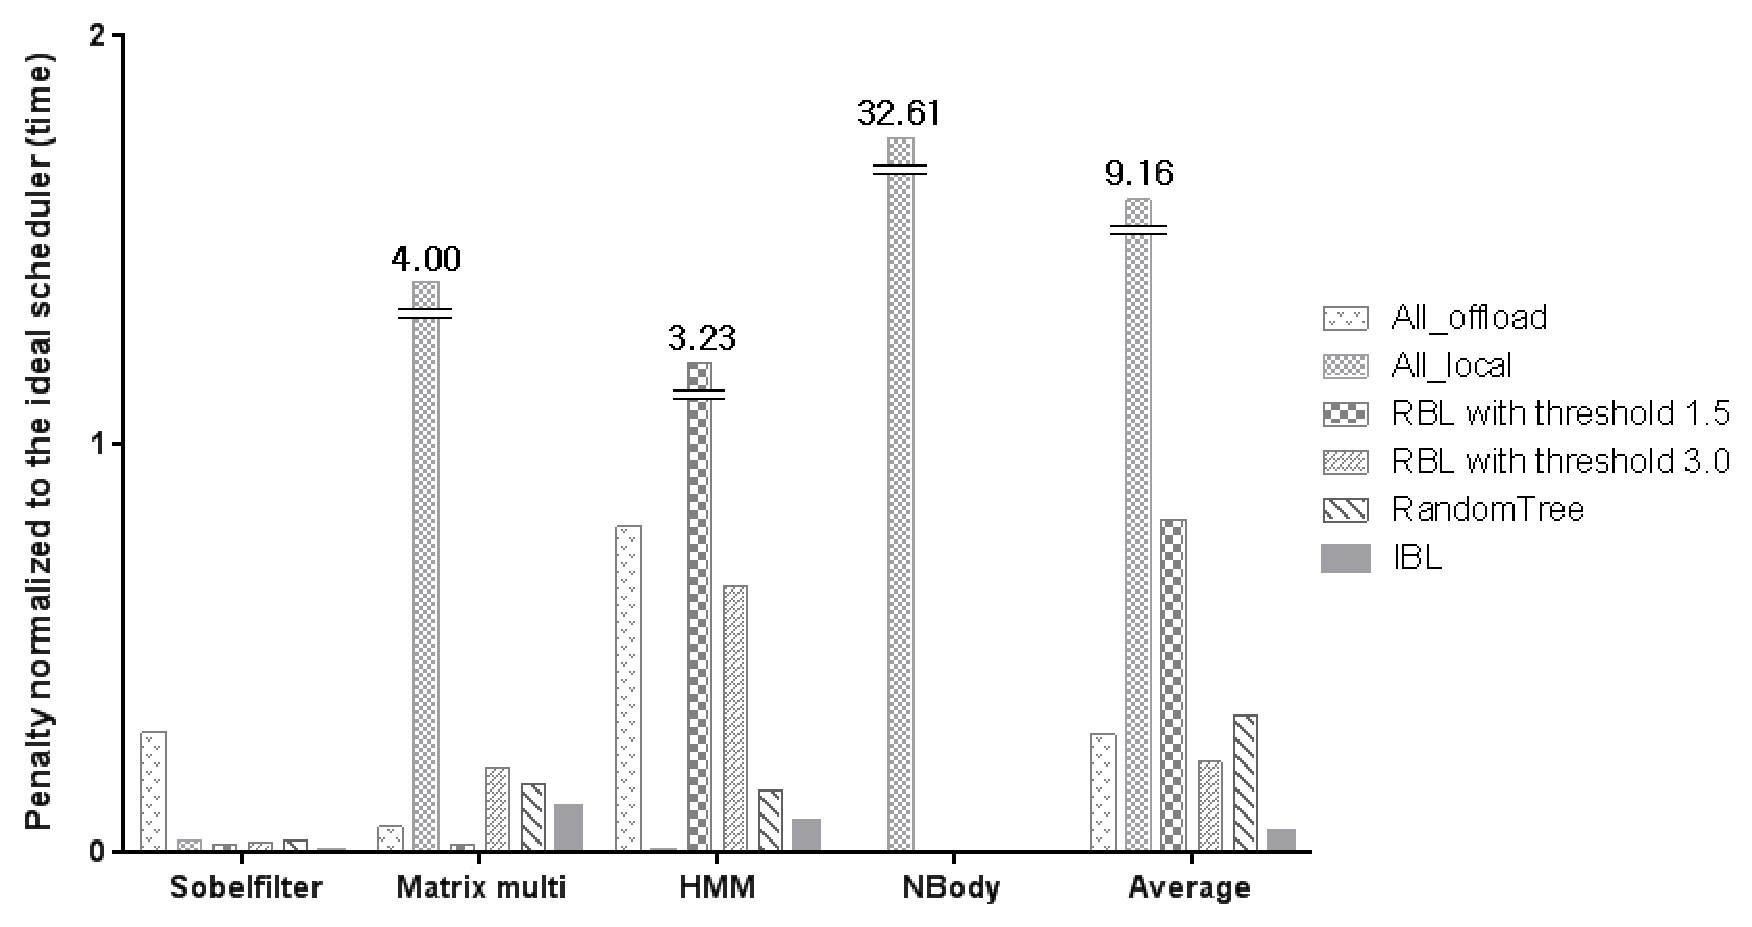
\epsfig{file=figs/penalty_time.eps, width=5.5in}
\caption{Penalty(execution time) normalized to the oracle scheduler}
\label{fig:penalty_time}
\end{figure}
%
\begin{figure}
\centering
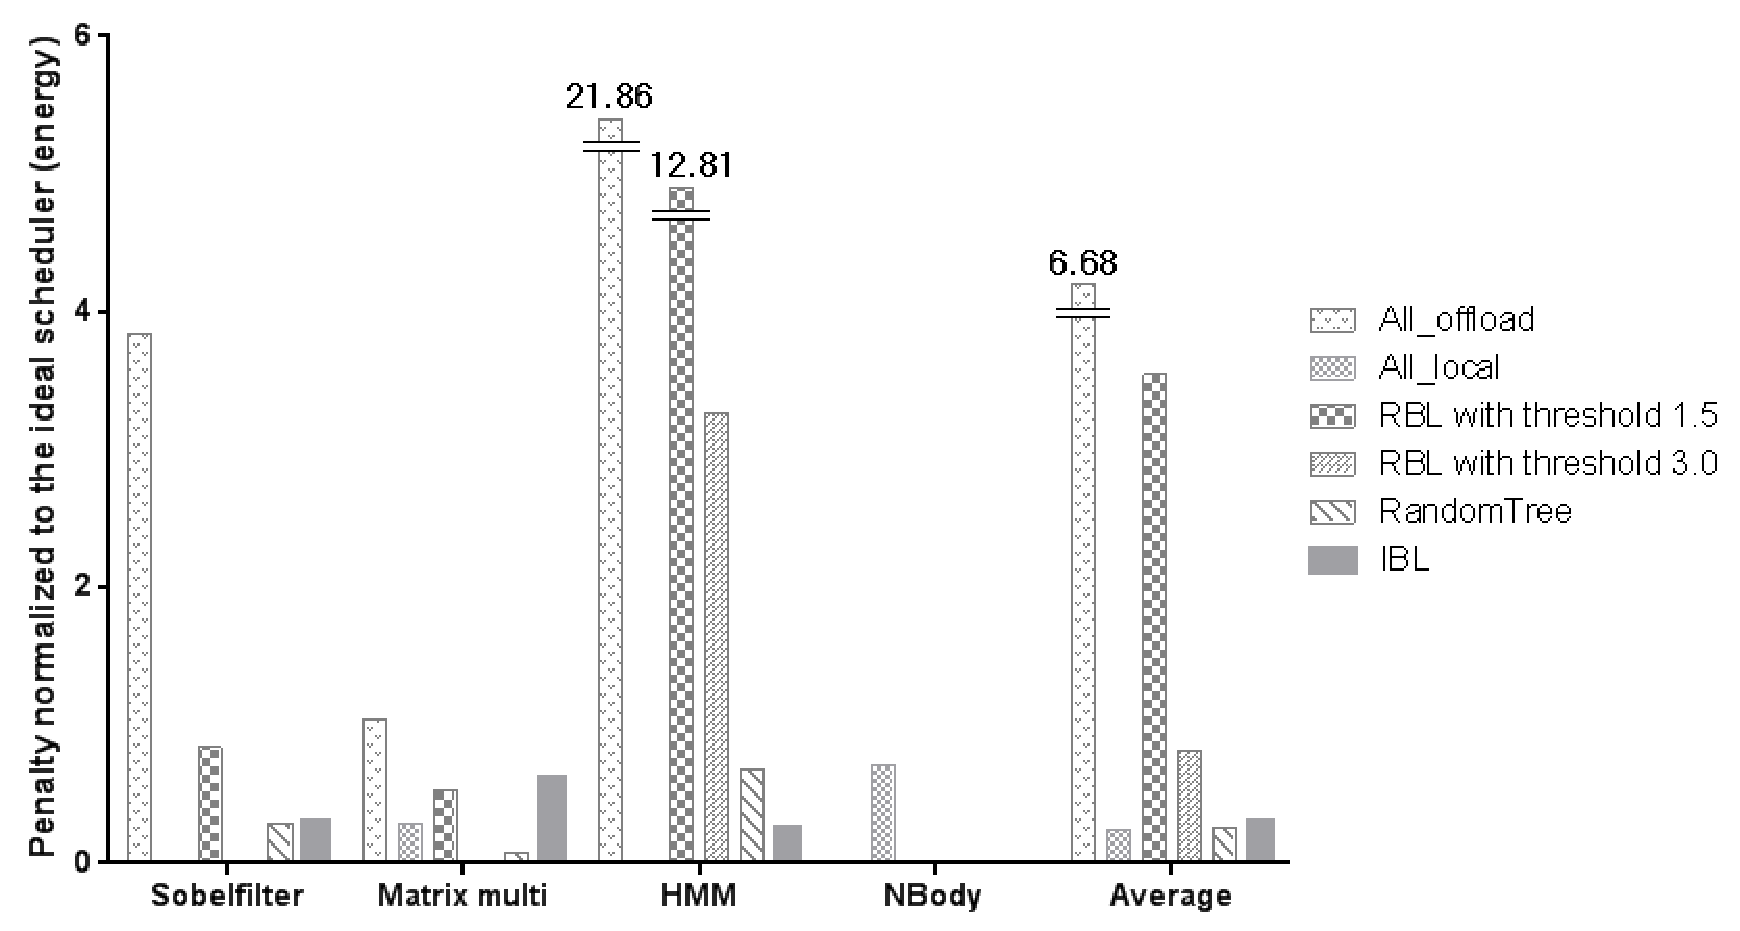
\epsfig{file=figs/penalty_energy.eps, width=5.5in}
\caption{Penalty(energy consumption) normalized to the oracle scheduler}
\label{fig:penalty_energy}
\end{figure}
%
\begin{equation}
\begin{split}
	penalty_{normalized} \\ 
		&	= (execution\_time_{ML} 
               - execution\_time_{oracle}) \\
        &        / execution\_time_{oracle}
\end{split}
\label{equ:penalty}
\end{equation}
%
where {\it execution\_time$_{ML}$} and 
{\it execution\_time$_{oracle}$} are the processing times 
of the workload scheduled by the machine learning-based scheduler 
and the oracle scheduler, respectively.
%
For the penalty in terms of energy consumption, 
{\it execution\_time$_{ML}$} and {\it execution\_time$_{oracle}$}
should be replaced with the mobile device's energy consumption to 
execute or offload the workload scheduled by each scheduler.
%
In this evaluation, the penalty implies the extra costs that the mobile
device or user has to pay additionally over the oracle scheduler when
the machine learning-based scheduler makes a wrong decision. 
%
To profile energy consumption of the mobile device, I used
PowerTutor~\cite{powertutor} which is an application for the variants of
Android devices that displays the power consumed by major components
such as CPU, network interface, LCD display, and GPS receiver.\\
%
As you can see, the Instance-Based Learning scheduler has the smallest
penalty in terms of the execution time because it has the highest
scheduling accuracy.
%
For energy consumption, moreover, the Instance-Based Learning scheduler has
a fairly small penalty compared with Rule-Based Learning scheduler.
%  
Note that, for sobelfilter, the penalty in terms of both the execution
time and energy consumption is lower than other execution kernels,
because the gap of the execution time and energy consumption for
sobelfilter between offloading and the local execution is relatively
small.
%
Therefore, the penalty for sobelfilter is less significant than the
cases of other execution kernels when the scheduler makes a wrong
decision on offloading or the local execution.
%

\section{Online Runtime Scheduler}
\label{scheduler:online}
%
In the previous section, I demonstrated the offline runtime offloading
scheduler based on various machine learning algorithms by illustrating
the scheduling accuracy and the penalty with regard to the execution
time and energy consumption of the mobile platforms.
%
In this section, I explore the potential possibility and benefits of an
online runtime scheduler for mobile offloading framework in which
the online scheduler can be trained through the previous experiences
automatically and adapt to the dynamic situation.
%
\subsection{Implementation of the Online Offloading Scheduler}
\label{scheduler:online_impl}
%
I first implemented the prototype of the online runtime scheduler
based on the Instance-Based Learning algorithm for the mobile offloading
framework.
%
The reason why I chose the Instance-Based Learning algorithm for the
online runtime scheduler is due to the simplicity of the algorithm and
the ability to quickly apply newly seen data to its future decisions.
%
Usually, other machine learning algorithms such as neural networks or
linear regression have its own the classification model and it is
required to be completely modified when a new instance data is added to
the training dataset.
%
However, Instance-Based Learning simply stores the new instance to the
training dataset, and the new instance is used to predict a next coming
problem instance along with previous stored instances.
%
In addition to its simplicity, in the evaluation for the offline offloading scheduler,
Instance-Based Learning showed the best performance among various
machine learning algorithms I used for the evaluation.\\
%
The following is the scheduling process of our prototype of the online
scheduler.
%
Once the application starts, the online scheduler executes the
application locally at once to figure out the information which is
required for profiling the workload such as the local execution time, the
size of data, or the number of the invocations for argument setup.
%
Then, the scheduler enters the training phase by unconditionally
offloading the execution to the remote server {\it N} times, and
each case is labeled according to the performance comparison between
offloading and the local execution.
%
The labeled instance is stored into the training database.
%
For the prototype, I set {\it N} with 16.
%
After the training phase, the scheduler starts the scheduling process by
measuring the Euclidean distance between a new scheduling problem and
the instances stored in the training database.
%
When offloading is scheduled, the scheduler offloads the workload and 
measures the execution time for offloading.
%
If offloading takes shorter than the local execution, then that instance
is added to the training database as {\it offload}.
%
On the other hand, it is stored as {\it local}.\\
%
To update the training database, the scheduler keeps adding the
new instance to the database without removing any previous stored
instance until the database is full.
%
Only if the database is full, the oldest instance will be replaced with
the new one.
%
For the implementation, I try to find the optimal number of instances for
the database which covers as many cases as possible, but takes reasonably small 
memory space (less than 1MB) and time (less than 0.01sec) to schedule a
new problem.
%
I chose 5,000 instances database which requires only 0.1MB of memory.
%
This memory usage occupies only less than 0.0007\% of typical memory
sizes of
contemporary mobile devices (e.g 16GB or 32GB).
%
Also, even though it takes 5$\sim$6msec to measure the Euclidean
distance of the new scheduling problem with 5,000
instances, I believe that instance generalization or clustering techniques for
the database such as~\cite{domingos, chang} can help the
scheduler significantly reduce the measurement time. 
%

\subsection{Evaluation for the Online Offloading Scheduler}
\label{scheduler:online_eval}
%
\begin{figure}
\centering
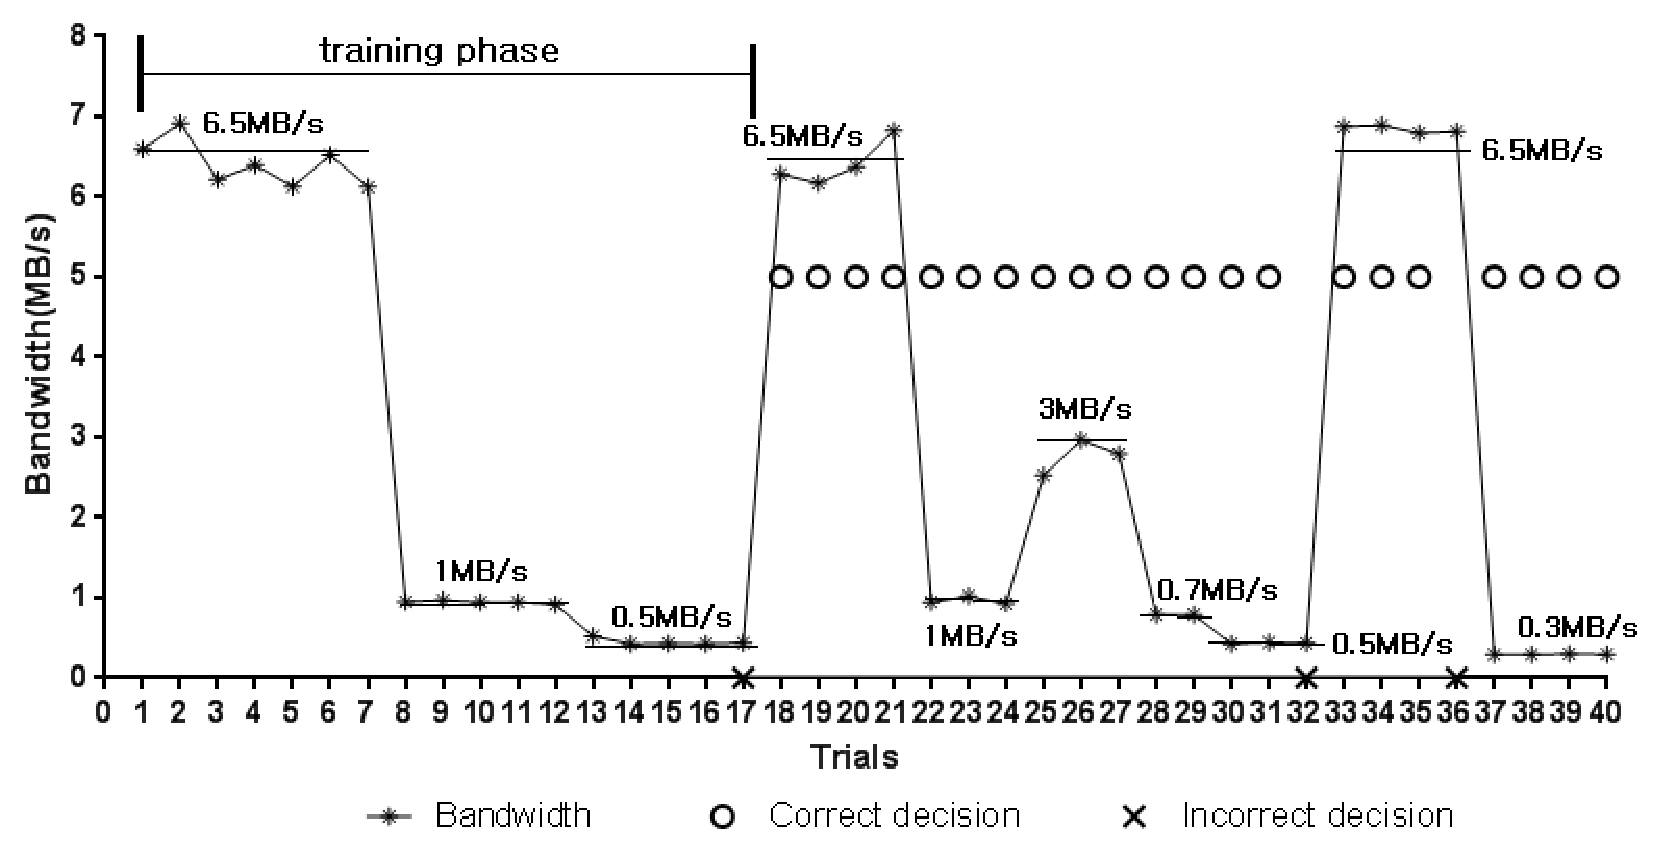
\epsfig{file=figs/online.eps, width=5.5in}
\caption{Adaptability of the online scheduler against dynamic network
conditions}
\label{fig:online}
\end{figure}

%
In order to evaluate the prototype of our online scheduler, I conducted
an experiment in which I change network conditions and observe how
well the scheduler learns and adapts to dynamic network conditions.
%
In this experiment, the client and the remote server are directly
connected through a wireless router and I controlled the network
bandwidth between them using TC.
%
Also, I used sobelfilter for the offloaded execution kernel.
%
Figure~\ref{fig:online} shows the ability to adapt the online scheduler to dynamic
network conditions.\\
%
\indent During the training phase, I setup different network conditions where
the scheduler is trained with three network bandwidths: 6.5MB/s, 1MB/s,
and 0.5MB/s.
%
After the training phase, the scheduler makes a decision on offloading
or the local execution in six different network bandwidths as shown in
Figure~\ref{fig:online}.
%
As you can observe, the scheduler makes the correct decisions in dynamic
network conditions except for 17th, 32nd, and 36th trial.
%
These incorrect decisions are because network bandwidth is changed
after the scheduler makes a decision.
%
As a result, the actual cost for data transfer is different with what
the scheduler predicts. 
%
Furthermore, even at the unseen conditions in the training phase such as
3MB/s or 0.3MB/s, the scheduler works correctly by making right
decisions.
%
Consequently, I observed the possibility and the potential benefits of
machine learning-based online offloading scheduler in this experiment. 
%
\section{Summary}
\label{scheduler:summary}
%
In this section, I proposed machine learning-based runtime scheduler for
mobile offloading framework.
%
Before addressing the scheduling problem of the mobile offloading
framework, I performed detailed measurement experiments under various
network conditions and mobile applications to show the necessity and
efficacy of an adaptive offloading mechanism.\\
%
In order to examine the feasibility of applying machine learning
techniques to the adaptive scheduling problem, I utilized Weka which is
a Java-based open source package.
%
To this end, I used computation to communication ratio, which represents
the local processing time for the workload, the amount of data transfer,
and network bandwidth, as an attribute of the machine learning
technique.
%
After investigating the scheduling accuracy of several machine learning
algorithms using Weka, I choose a few machine learning algorithms which
have relatively high scheduling accuracy to implement an offline
offloading scheduler.
%
In the evaluation, I showed that although Instance-Based Learning 
offloading scheduler is fairly simple and has low overhead, it provides
performance advantages over non-adaptive scheduling policy or even
another machine learning algorithm-based schedulers such as RandomTree
or Rule-Based Learning.
%
In fact, the scheduler based on Instance-Based Learning
performed 7\% better than RandomTree and 3\% better than Rule-Based
Learning.\\
%
Furthermore, by taking the complexity and scheduling performance into
account, I selected Instance-Based Learning algorithm for an online
scheduler for mobile offloading framework.
%
Using Instance-Based Learning online scheduler, I demonstrated
the potential benefits and the ability of the online offloading
scheduler to adapt into dynamic network conditions.
%
